 %PRE-PROCESSING ______________________________________________________________________
\documentclass{article}
\usepackage[english]{babel}
\usepackage[utf8]{inputenc}
\usepackage{johd}
\usepackage{dutchcal}
%\usepackage{pdfpages}
%\nonfranchspacingf

%RUBRIC ______________________________________________________________________
%RUBRIC HERE
%TITLE PAGE______________________________________________________________________
\pagenumbering{gobble} %Removes the Numbering on the first page


\title{Department of Chemical Engineering \linebreak
University of California, Santa Barbara \linebreak
\linebreak \linebreak \linebreak \linebreak
\linebreak \linebreak \linebreak
Chemical Engineering 180A \linebreak
Analysis of CO{{\textsubscript{2}}} and He Compressibilty at High Pressures \linebreak \linebreak \linebreak \linebreak
\linebreak \linebreak \linebreak \linebreak \linebreak \linebreak}

\author{Wesley Johanson, Chase Hartsell, Qiye Hu \\ 
        University Of California, Santa Barbara \\
        Group 3W\\
        Conducted from April $20^{th}$ - $27^{th}$, 2022
}



%BEGIN DOCUMENT ______________________________________________________________________
\begin{document} \maketitle \noindent 
\clearpage \pagenumbering{arabic} % Starts the numbering, using arabic symbols 1,2, etc.

%ABSTRACT ______________________________________________________________________
\section*{Abstract}

Gaseous compressibility is a key consideration for accurate engineering calculations in many applications. In this report, the compressibility factors of CO{\textsubscript{2}} and helium were investigated using Burnett's isothermal pressure ratio method at 10{\textsuperscript{o}}, 20{\textsuperscript{o}}, and 30{\textsuperscript{o} C}. The compressibility factor Z{{\textsubscript{CO{{\textsubscript{2}}}}}} was found to have a decreasing linear trend with increasing pressure, with the lowest value Z = 0.6 +/- 0.02 at 760 psi, and the system became more ideal with Z = 1 +/- 0.08 as pressure decreased to atmospheric. Helium exhibited ideal behavior, with Z{\textsubscript{He}} being relatively ideal with Z = 1 +/- 0.1 regardless of pressure. Although no significant deviations from ideality were observed from helium gas, there is a slight positive deviation with temperature increase, showing a temperature dependence in the second virial coefficient B(T) in helium gas, in addition to CO{\textsubscript{2}}. The second virial coefficients, which deviated by 50-100\% from literature values, increased non-linearly with temperature, and were negative for temperatures below 20{\textsuperscript{o} C} for helium and at all temperatures measured for CO{\textsubscript{2}}. CO{\textsubscript{2}}'s decreasing compressibility factor with pressure highlights the implications of non-ideality in gases, and the calculations for CO{\textsubscript{2}} wouldn't be as accurate at same temperature and pressure as its ideal counterpart helium. 

%INTRODUCTION _____________________________________________________________________
\section*{Introduction} 
With recent world events and supply chain issues, supply storage has became a major concern in the United States. Many vital instruments, like MRI machines in hospitals, require liquid helium for cooling purposes. However, with the recent turmoil in one of the world's major helium suppliers, helium has become scarce[1] and this shortage could potentially derail scientific and medical research. In lieu of this, finding new compressible gasses may prove to be important for future applications in this sense.
\noindent The goal of this report is to find the compressibility factor Z for gases CO$_2$ and Helium, and to create a solid model for z at different temperatures.
 The pressure, molar volume, and temperature of a gas are related by the equation of state:
\begin{equation} \label{eq:1} Z=\frac{PV}{nRT} \end{equation}

 \noindent where R is the universal gas constant. The compressibility factor, Z, is a unit-less measure of gas ideality (ideal gas has Z =1), and it can be determined for different gasses at different conditions.
 Factors that affect gas ideality include inter-molecular forces and molecular size. Because of this, ideal behavior is observed at high temperatures and low pressures, when these two effects are minimized.
 \linebreak To measure the compressibility factors of carbon dioxide and helium, we employed Burnett’s method[2] and observed the change in pressure as a gas was expanded at a constant temperature. 
 By relating the change in pressure after the r$^{th}$ expansion to a consistent change in volume (represented by the apparatus constant, N), the deviations from ideal expectations can be measured.
 
\begin{equation} \label{eq:1} \frac{p_{r-1}}{p_{r}} = N\frac{Z_{r-1}}{Z_{r}} \end{equation}
Because gas acts closest to ideal at low pressures, taking the limit as pressure goes to zero allows us to solve for the apparatus constant. Using this, a relation can be developed between the ratio in pressures after an expansion to the ratio in compressibility factors. We can then calculate Z from the initial and current pressure at any given expansion.

\begin{equation} \label{eq:2} 
p_{r}N^{r} = \left(\frac{p_{0}}{Z_{0}}\right)Z_{r}
\end{equation}
Because compressibility is also affected by temperature, a linear model can be generated to obtain Z as a function of pressure at each isotherm. The slope of this line is the temperature dependent B'; the intercept, at zero pressure, is Z=1: an ideal gas.
\begin{equation} \label{eq:3} Z=1+B'P \end{equation}

\noindent From the slope of compressibility factor B', the second virial coefficient can be obtained from B' through equation[3]: 
\begin{equation} \label{eq:4} B(T) = B'* RT \end{equation}
However, due to unique  molecular structures, the compressibility and second virial coefficient would deviate from ideal state as pressure increases. This is due to multiple factors from intermolecular forces. The attractive and repulsive behavior between the pure gas molcules, like the Van der Waals forces, would affect how ideally a molecule like methane would behave under a set temperature and pressure[4].    

%EXPERIMENTAL______________________________________________________________________
\section*{Experimental Methods}

\begin{figure}[H] \centering
\includegraphics[width=0.8\textwidth]{images/APPARATUS.PNG}
\caption{\label{fig1} Pressure vessel apparatus where gas was expanded and the pressure was recorded after it reached equilibrium.}\end{figure}

The apparatus (Figure 1)consists of a high purity gas source (He and CO\textsubscript{2}, Airgas, 100\%). The high purity gas source is connected to two interconnected vessels, one of which is attached with a pressure indicator (PI) and the other to vent and vacuum. All the connections connected to the vessels are regulated with a manual gate valve, with the whole apparatus taking place in a temperature controlled (TC) water bath.%LINE

The goal of this experiment is to use Burnett's method to find the compressibility factor Z of gases He and CO\textsubscript{2}, at different pressure and temperature. A source gas, CO\textsubscript{2} or He, is introduced into the vacuumed vessel 1 via opening valve 1. %LINE

Once the set pressure is reached in vessel 1, valve 1 is closed and valve 2 is opened slowly to allow gas to expand into the vacuumed vessel 2 isothermally. Once the pressure equalized, it is recorded and valve 2 is closed and the gas in vessel two is vented out via valve 3 and vacuumed via valve 4. After vessel 2 is vacuumed, valve 2 is reopened for another expansion. Expansions are repeated until the equilibrium pressure approaches atmospheric pressure, or the measurement is too low to accurately read.
\linebreak \noindent With the expansion data at different temperature, the compressibility factor can be calculated via equation 2 and 3, thus a pressure dependent compressibility value Z graph is made (Figures 2 \& 3). The slope of the Z graph is the temperature dependent second virial coefficient, which is graphed at the three temperatures measured (Figure 4).  

%RESULTS______________________________________________________________________
\section*{Results and Discussion}
The Z factors as a function of pressure for helium and carbon dioxide (Figures 2 \& 3), exhibit a linear dependence in this pressure range. Values for raw pressure readings used to calculate Z are located in Tables 1 \& 2 in Appendix A. The compressibility factor for helium does not have a clear trend with increasing pressure. There is imprecise correlation between pressure and the Z factor given by the low R{\textsuperscript{2}} values at three different temperatures, however the error bars suggest relative ideality with Z = 1 +/- 0.1 (Figure 2). \linebreak Gas is most ideal at high temperatures and low pressures, however the 30{\textsuperscript{o}} isotherm exhibits the most deviation from ideal behavior, even outside of the error range for most measurements. ADD MORE

\begin{figure}[H] \centering
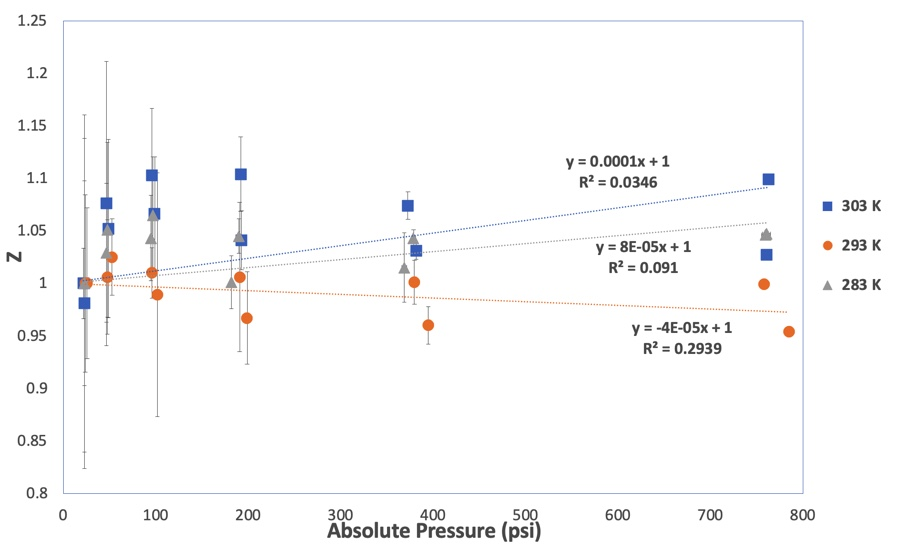
\includegraphics[width=.8\textwidth]{images/ZvsP Helium.jpg}
\caption{\label{fig1}Compressibility of helium at 3 isotherms. Error bars represent standard error of calculations and pressure gauge readings.}\end{figure}

\noindent The seemingly unpredictable points shown in Figure 2 can be explained by Helium's inert nature. Due to helium's monoatomic and stable nature from filled orbitals, helium atoms have no attraction towards each other, making it inert. Helium is also the second smallest atom, so the volume of the container is a very fair estimate for the volume of empty space, whereas the larger carbon dioxide makes a more significant effect on this assumption. This explains the ideal behavior seen in Figure 2. Even with the imprecise distribution, Z{{\textsubscript{He}}} has a value of relatively one across all pressures. This is similar to Imbert's Z value of 1 + 0.0045 P(MPa)[5]. The cause of the high spread in these values, especially at lower pressures, is because error in the pressure readings gets propagated through after each expansion. In addition to this, the gauge was accurate to +/- .25\%, and this systematic error also becomes more significant at lower pressure readings. Because helium was so close to ideal, these deviations look like a large spread with little correlation however the error bars suggest a linear pressure dependence at these conditions. \linebreak
\linebreak
In addition to helium, a trend for Z{{\textsubscript{CO{{\textsubscript{2}}}}}}'s compressibility is also reasonable. However, the Z factors for carbon dioxide show a stronger pressure dependence, decreasing linearly in this temperature and pressure range (Figure 3). CO{{\textsubscript{2}}}'s bonds provided the molecule with a net zero dipole, but compared to helium's inert nature, CO{{\textsubscript{2}}} experiences  bigger Van der Waals forces due to the instantaneous dipole moment given by a more electronegative oxygen atom at each end. This means that when a molar charge is introduced into a constant volume, CO{{\textsubscript{2}}} gas molecules experience a stronger attractive force, exhibiting a lower pressure than ideal and thus having a lower Z value at these pressures. The trends shown in Figure 3 also match with Sage and Lacy (1955) and Burton Technical Bulletin (1990) data showing a negative linear slope in the Z factor until 1500 psia at 100{\textsuperscript{o}}F[6]. Experimental data also shows the same negative slope, with the similar Z values within 4\%. Experimental data also displays ideal gas trends, with the higher temperature exhibiting the most ideal behavior.

\begin{figure}[H] \centering
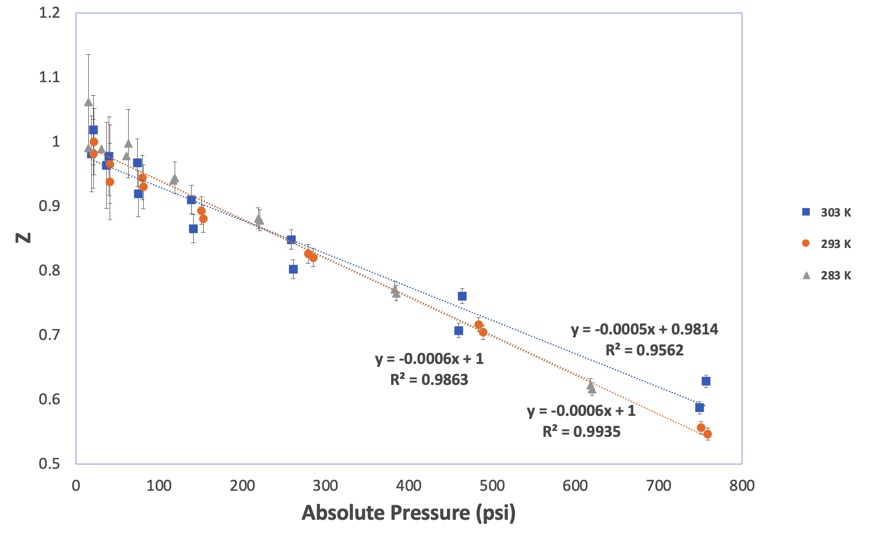
\includegraphics[width=.8\textwidth]{images/ZvsP Co2.jpg}
\caption{\label{fig1}Compressibility of carbon dioxide at 3 isotherms. Error bars represent standard error of calculations and pressure gauge readings.}\end{figure}
\noindent
A key difference in the Z factor determination between helium and carbon dioxide gas is that carbon dioxide would readily liquefy under high pressure. From the CO{{\textsubscript{2}}} phase diagram, CO{{\textsubscript{2}}} liquefies at 30{\textsuperscript{o}}C and 760 psi, and at 10{\textsuperscript{o}}C it liquefies at 650 psi. This prevented us from charging the vessel with as much gas, and one less expansion was able to be precisely measured at 10{\textsuperscript{o}}C. ADD MORE\linebreak \linebreak
\noindent After obtaining experimental data for the compressibilty factors of each gas, a linear regression model was set up, with the intercept set at the ideal Z = 1. Using this isothermal variation of the pressure ratio method to determine Z factors, the slope of these lines (Figure 4) are the second virial coefficients, which are dependent on temperature[7]. ADD MORE, explain values and comparison/physical stuff that affects B

\begin{figure}[H] \centering
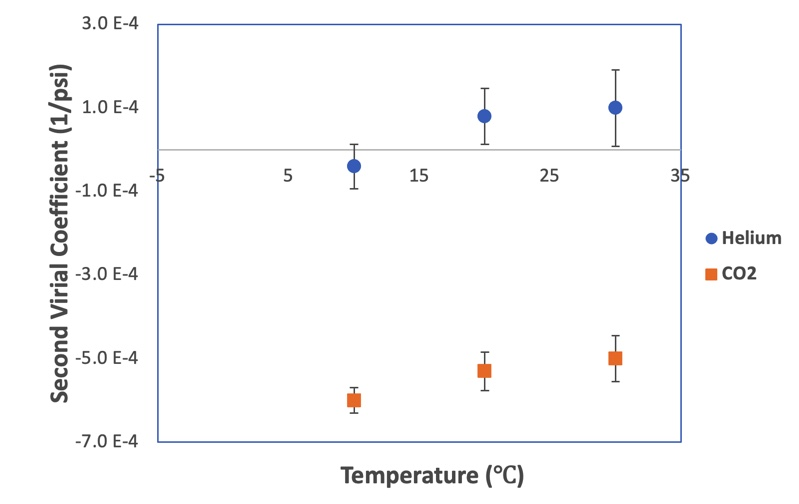
\includegraphics[width=1\textwidth]{images/NewB.jpg}
\caption{\label{fig1}The second virial coefficients of helium and carbon dioxide at the three temperatures that were measured. Error bars represent standard error of the values calculated over two trials of six expansions at each isotherm.}\end{figure}

\section*{Conclusion}
The chemical make-up of a gas affects how compressible it is under high pressure. CO{{\textsubscript{2}}}'s compressibility decreased with increasing pressure at all three isotherms. The compressibility factor Z{{\textsubscript{CO{{\textsubscript{2}}}}}} has decreased down to almost 0.6 at 750 psi, meaning that at same pressure and volume, CO{{\textsubscript{2}}} contains 40{\%} more moles than helium according to equation 1. The decrease in Z{{\textsubscript{CO{{\textsubscript{2}}}}}} is a result of the Van der Waals attraction between the molecules, and as molecules being compressed, they would have less expulsion forces between each other as experienced on helium gas. In addition, CO{{\textsubscript{2}}} is a significantly larger molecule than monoatomic helium, and the fact that a vessel of CO{{\textsubscript{2}}} has less empty space between the gas particles than helium has implications on its compressibility.
%REFERENCES  ______________________________________________________________
\newpage \section*{References} 
1. Helium shortages return. (2022). C\&EN Global Enterprise, 100(6), 9–9. doi:10.1021/cen-10006-buscon4

2. Silberberg, I. H., Kobe, A. K., McKetta, J. J.(1959). "Gas Compressibilities with Burnett Apparatus." J. Chem. Eng. Data 4, 314-329 

3.Hajjar, Raja Faris. “THE DETERMINATION OF THE SECOND VIRIAL COEFFICIENTS AND THE MOLECULAR CONSTANTS OF SIX HALOGEN-SUBSTITUTED METHANES BYU A GAS BALANCE METHOD.” The Ohio State University, 1967.

4.Schamp, Jr, H W, Mason, E A, Richardson, A C.B., and Altman, A. COMPRESSIBILITY AND INTERMOLECULAR FORCES IN GASES: METHANE. https://doi.org/10.1063/1.1705891

5. Imbert, G et al. “The compressibility and the capacitance coefficient of helium-oxygen atmospheres.” Undersea biomedical research vol. 9,4 (1982): 305-14. 

6. Adisoemarta, P et al. "Measurement of Z-Factors for Carbon Dioxide Sequestration." Texas Tech University.(2004). 

7. Berberan Santos, Mario N and Bodunov, Evgeny N. and Pogliani, Lionello. (2008). The van der Waals equation: Analytical and approximate solutions. Journal of Mathematical Chemistry. 43. 1437-1457. 10.1007/s10910-007-9272-4. 

8. Van Ness, H. C., Classical Thermodynamics of Non-Electrolyte Solutions, Pergamon Press, pp. 45-51 (1964).

9. Burnett, E. S. "Compressibility Determinations Without Volume Measurements." Journal of  Applied Mechanics. 3(4), A136-A140. (1936). 

10. Witonsky, J. R., Miller, G. J. (1963). “Compressibility of Gasses. IV. The Burnett Method Applied.” American Chemical Society. 

12. J. M. H. Levelt Sengers, Max Klein, and John S. Gallagher. (1971). "Tables of Second Virial Coefficients and Thier First and Second Derivatives for the Stockmayer (m,6,3) Potential Function." National Bureau of Standard and Physical Chemistry. 

13. Gallagher, S. J., Crovetto R. (1992). "The Thermodynamic Behavior of the Co2-H2O Sytsem from 400 to 1000K, up to 100 MPa and 30\% Mole Fraction of CO2." National Institute of Standards and Technology, 443.

14. Barth, Ginger. (2006). "Methane Gas Volume Expansion Ratios and Ideal Gas Deviation Factors for the Deep-Water Bering Sea Basins." U.S. Geological Survey.


%APPENDIX: RAW DATA ______________________________________________________________
\newpage \begin{centering}\section*{Appendix A: Raw Data} \end{centering}
Figure 4 displays how N, the apparatus constant, was experimentally determined. N is the ratio of final volume to initial volume for each expansion, and it was constant for each expansion. Vessel 1 and 2 theoretically had the same volume, so the apparatus constant was expected to be two, and the average of both gas's calibration proved this to be believable within the error range.

\begin{figure}[H] \centering 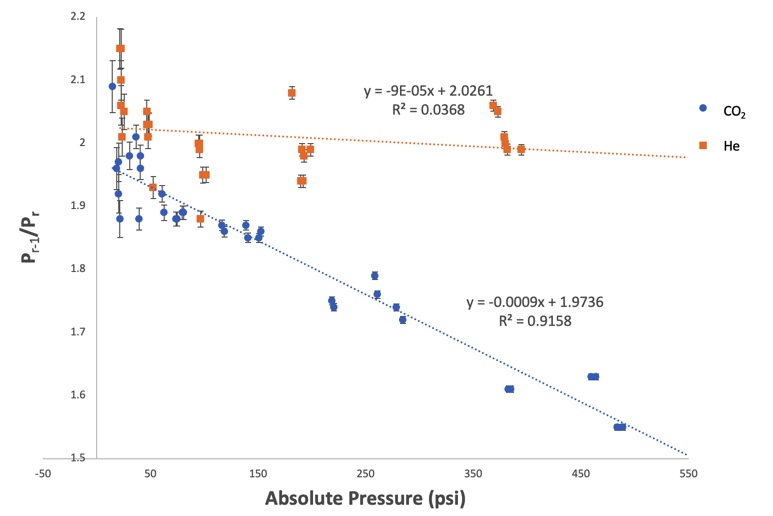
\includegraphics[width=0.8\textwidth]{images/N graph.jpg} \caption{\label{fig1}Calibration for the apparatus constant of the helium pressure vessel system. The limit as pressure approaches 0 (which is the y-intercept) determines the apparatus constant $N$ i.e. the ratio of $V_{r}/V_{r-1}$. This was determined on the same apparatus with helium and carbon dioxide, and the expected value is 2.}.\end{figure}

\noindent To determine $Z_{0}$ for each run, regression was used to find the limit of our data as gauge pressure approached zero. This gives the ratio of the $\frac{P_{0}}{Z_{0}}$, so that successive Z factors can be calculated using equation 6 (Appendix B).

\begin{figure}[H] \centering
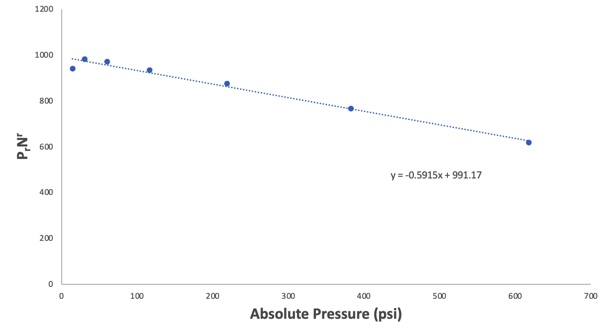
\includegraphics[width=0.8\textwidth]{images/NrPr.jpg}
\caption{\label{fig1}As $P_{r}$ approaches low pressures, the value of $Z_{r}$ approaches unity. The limit of this data set as pressure approaches atmospheric allows us to determine the value of $Z_{0}$ in equation 3. The data in this graph is from the 12th run (carbon dioxide at 283 K).}\end{figure}
\noindent

\newpage 
\caption{\label{fig1}Table 1: Raw pressure measurements for each successive expansion at a given temperature for He. Two series of five expansions were tested for each temperature.} 

\centering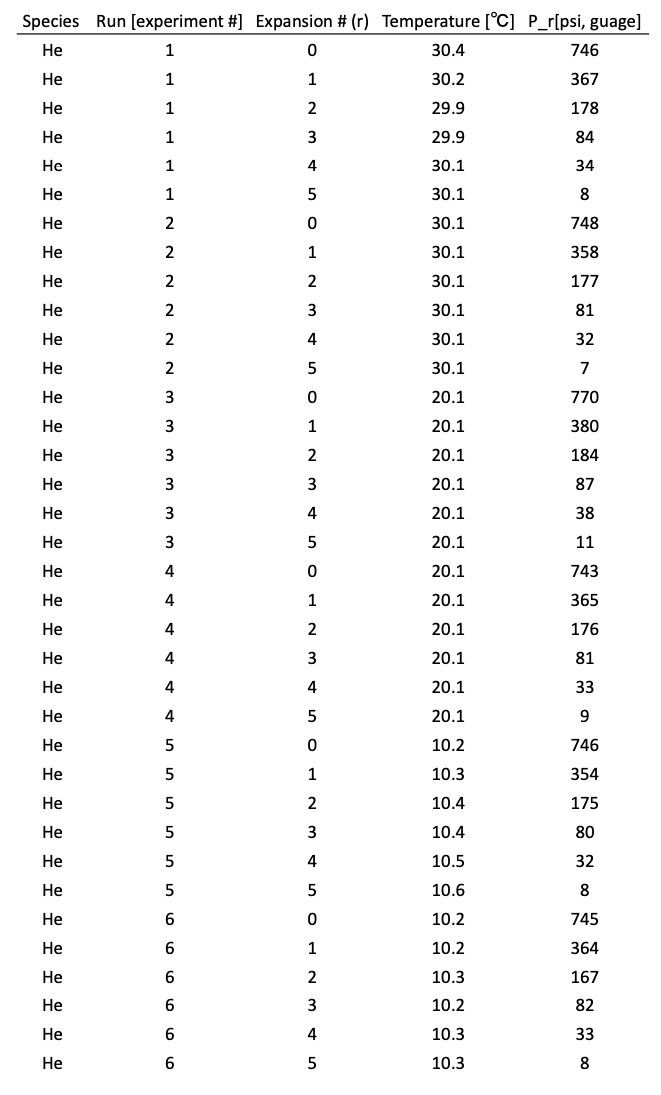
\includegraphics[width=0.5\textwidth]{images/table_0.png}\raggedright

\newpage \caption{\label{fig1}Table 2: Raw pressure measurements for each successive expansion at a given temperature for $C0_2$. Two series of six expansions were tested for each temperature.}
\centering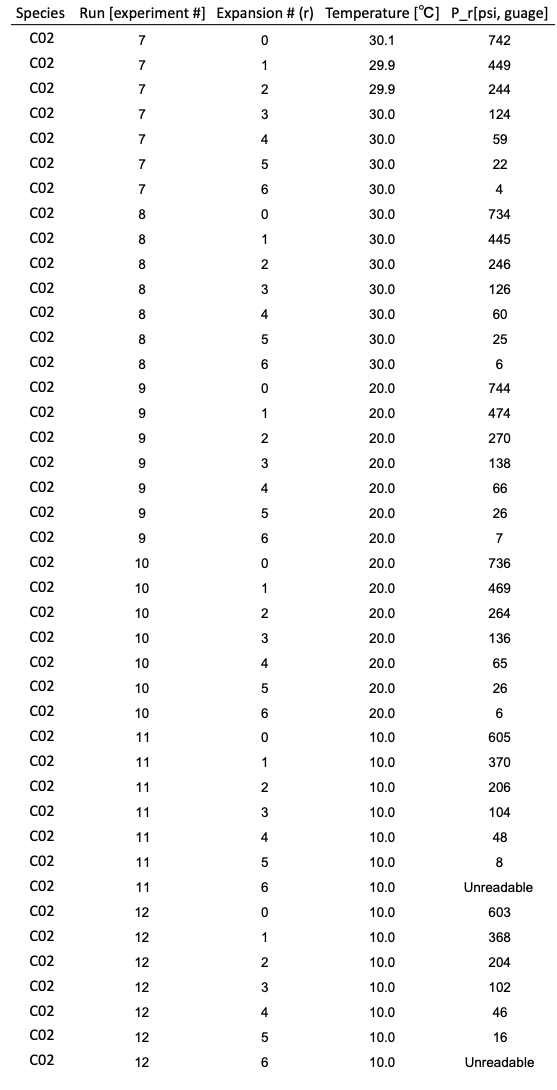
\includegraphics[width=0.5\textwidth]{images/table_1.png}\raggedright

\caption{\label{fig1}Table 3: Comparison of our second virial coefficient calculations with literature values}
\centering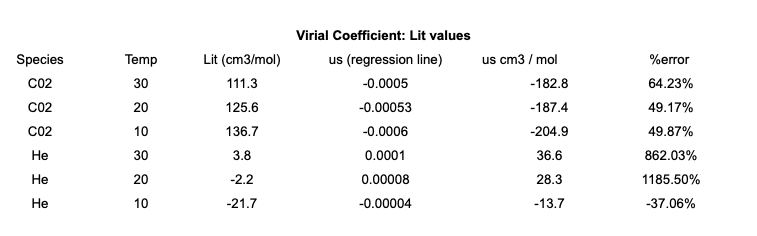
\includegraphics[width=0.5\textwidth]{images/b_error.png}\raggedright


%APPENDIX B ______________________________________________________________
\newpage \begin{centering} \section*{Appendix B: Sample Calculations} \end{centering}

For each subsequent expansion,
\begin{equation} \label{eq:1} 
\left(\frac{p_{r-1}}{p_{r}}\right) = N\left(\frac{Z_{r-1}}{Z_{r}} \right)
\end{equation}
this equation was used to determine the apparatus coefficient. As low pressures are approached, the gas behaves more ideally. Consequentially the ratio of $\frac{Z_{r-1}}{Z_{r}}$ approaches 1 and N will be the ratio of $\frac{p_{r-1}}{p_{r}}$ as seen in the limit.
\begin{equation} \label{eq:1} 
\lim_{p\to0} \left(\frac{p_{r-1}}{p_{r}}\right) = N
\end{equation}

\begin{equation} \label{eq:3} 
p_{r}N^{r} = \left(\frac{p_{0}}{Z_{0}}\right)Z_{r}
\end{equation}
This equation was used to find the value of $Z_0$. At low pressures, the value of $Z_r$ approaches unity since it behaves ideally. The value of $Z_0$ can be determined from the the ratio of the initial pressure and $P_rN^r$. \linebreak
\linebreak
Every value recorded for pressure was within .25\% of its true value according to the gauge, as well as a .5 psi uncertainty between the tick marks, and an estimate was made to best determine the observed pressure after each expansion. With this error, it gets bigger as we take the ratio of the pressure at each given expansion (calculated by the 'Multiplication or division' method).This error is carried through to calculating Z and B with the same method.

\begin{figure}[H] \centering
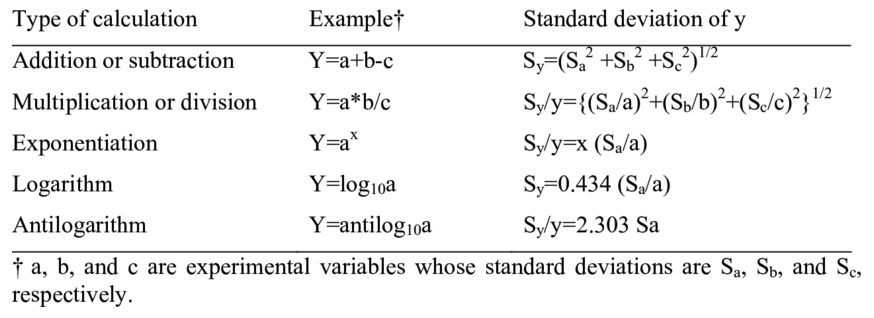
\includegraphics[width=0.8\textwidth]{images/error.png}
\caption{Error propagation was calculated using the methods on this chart. When combining two values with error, the propagation was kept through and error grew as we calculated Z factors for more and more expansions.
\label{fig1}}\end{figure}
    


%APPENDIX C ______________________________________________________________
\centering \section*{Appendix C: Program Files} 

\begin{figure}[H] \centering
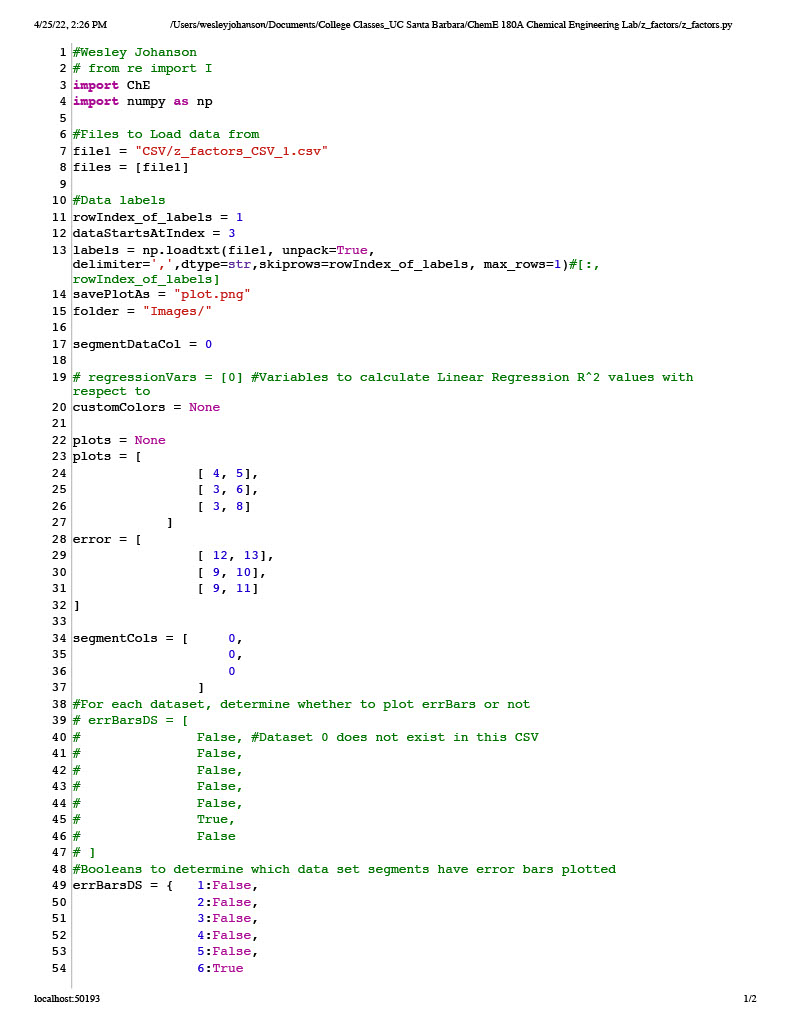
\includegraphics[width=0.8\textwidth]{code/z_factors_py1024_1.jpg}
\caption{\label{fig1}Primary logic/script: python code}\end{figure}


\begin{figure}[H] \centering
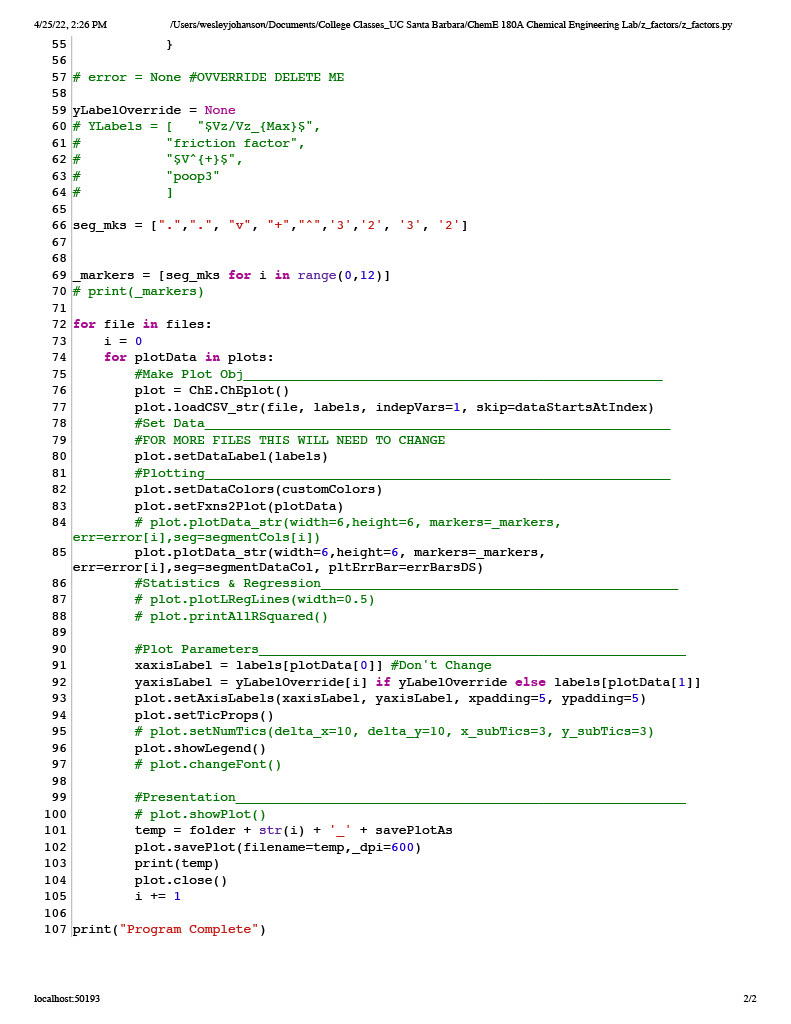
\includegraphics[width=0.8\textwidth]{code/z_factors_py1024_2.jpg}
\caption{\label{fig1}Primary logic/script: python code}\end{figure}

\begin{figure}[H] \centering
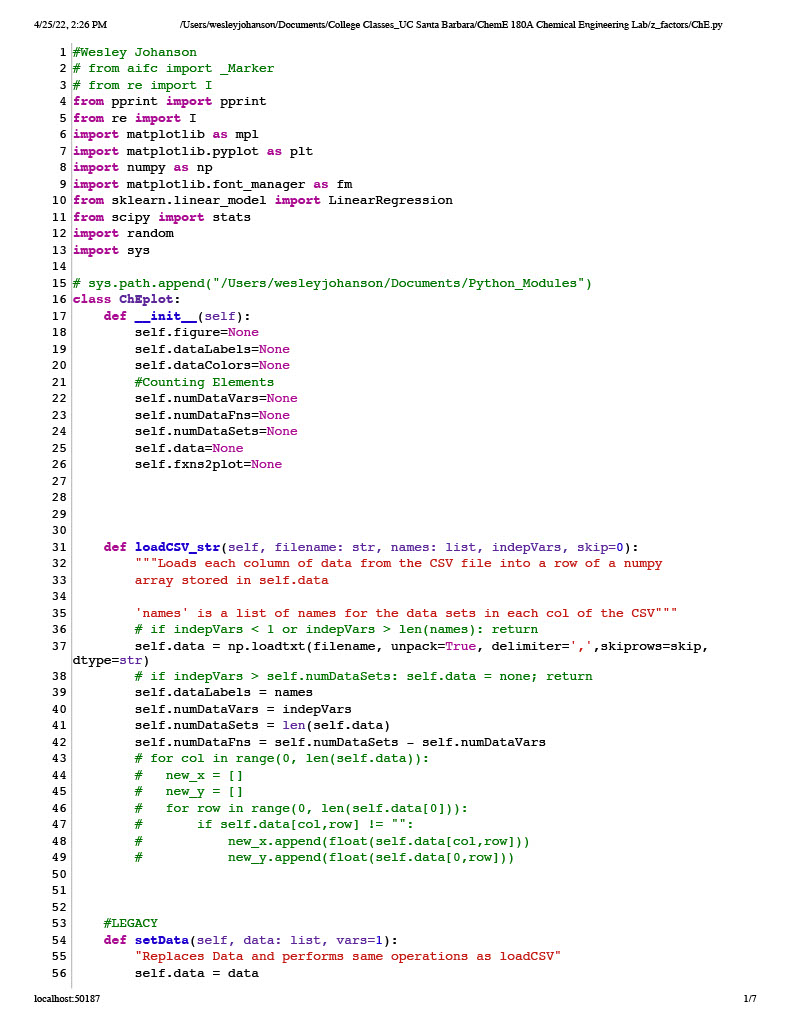
\includegraphics[width=0.8\textwidth]{code/che_py1024_1.jpg}
\caption{\label{fig1}Plotting Class python code}\end{figure}


\begin{figure}[H] \centering
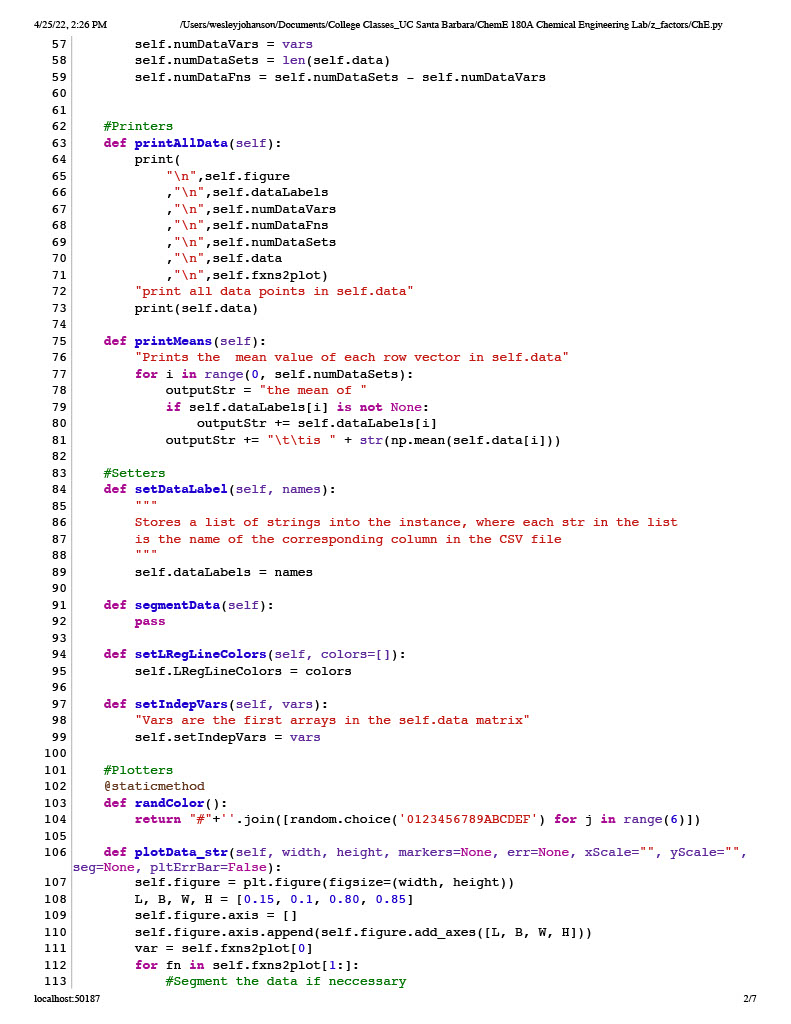
\includegraphics[width=0.8\textwidth]{code/che_py1024_2.jpg}
\caption{\label{fig1}Plotting Class python code}\end{figure}


\begin{figure}[H] \centering
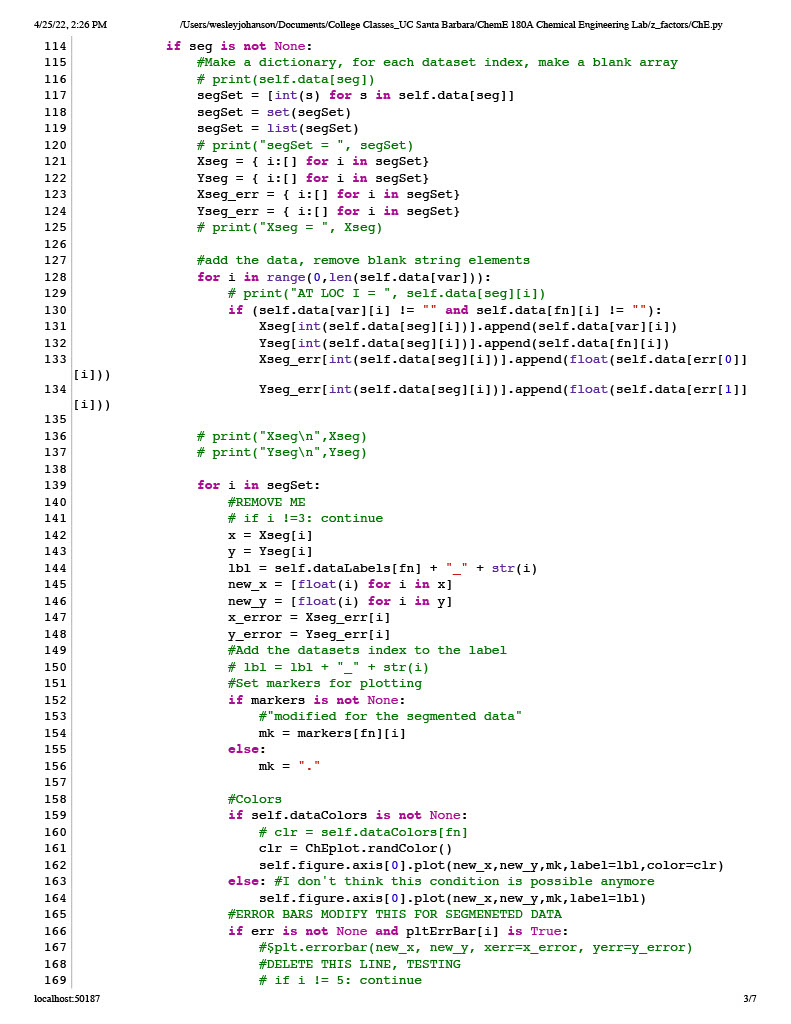
\includegraphics[width=0.8\textwidth]{code/che_py1024_3.jpg}
\caption{\label{fig1}Plotting Class python code}\end{figure}


\begin{figure}[H] \centering
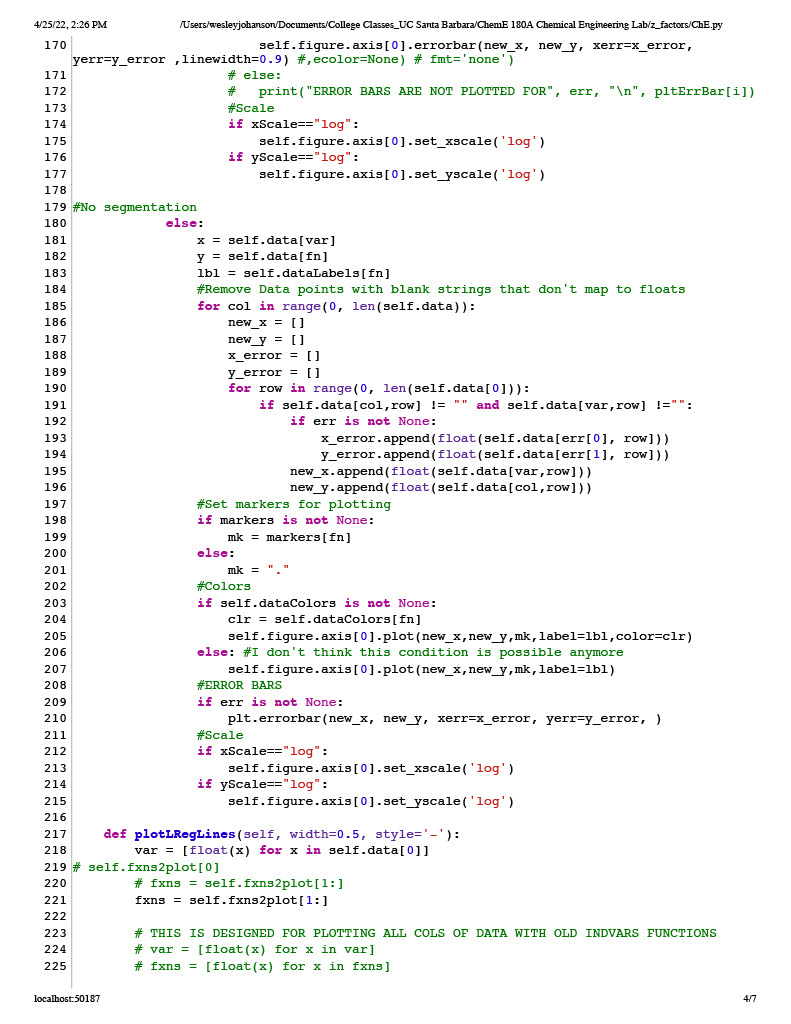
\includegraphics[width=0.8\textwidth]{code/che_py1024_4.jpg}
\caption{\label{fig1}Plotting Class python code}\end{figure}

\begin{figure}[H] \centering
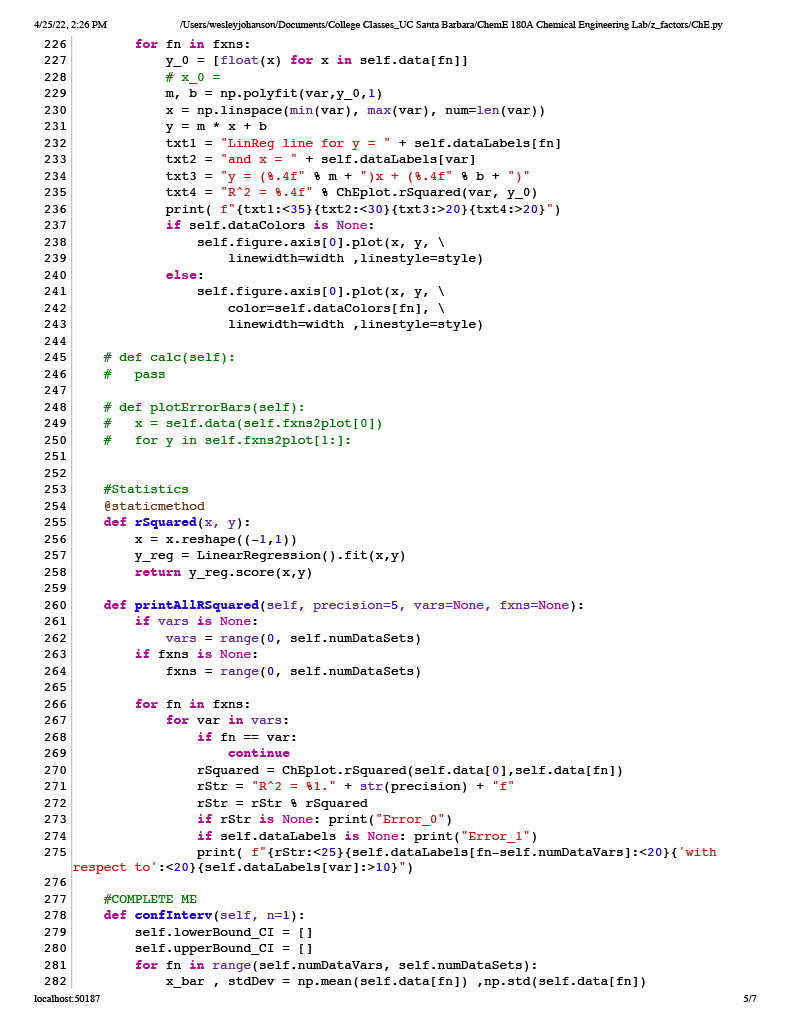
\includegraphics[width=0.8\textwidth]{code/che_py1024_5.jpg}
\caption{\label{fig1}Plotting Class python code}\end{figure}

\begin{figure}[H] \centering
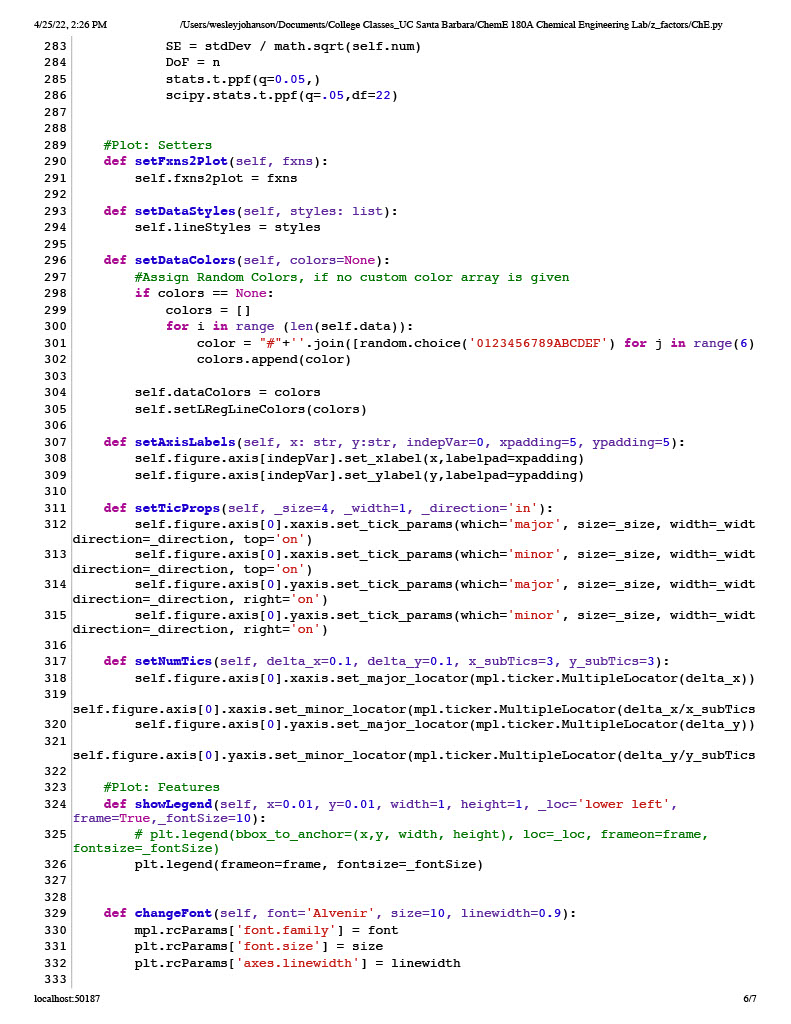
\includegraphics[width=0.8\textwidth]{code/che_py1024_6.jpg}
\caption{\label{fig1}Plotting Class python code}\end{figure}

\begin{figure}[H] \centering
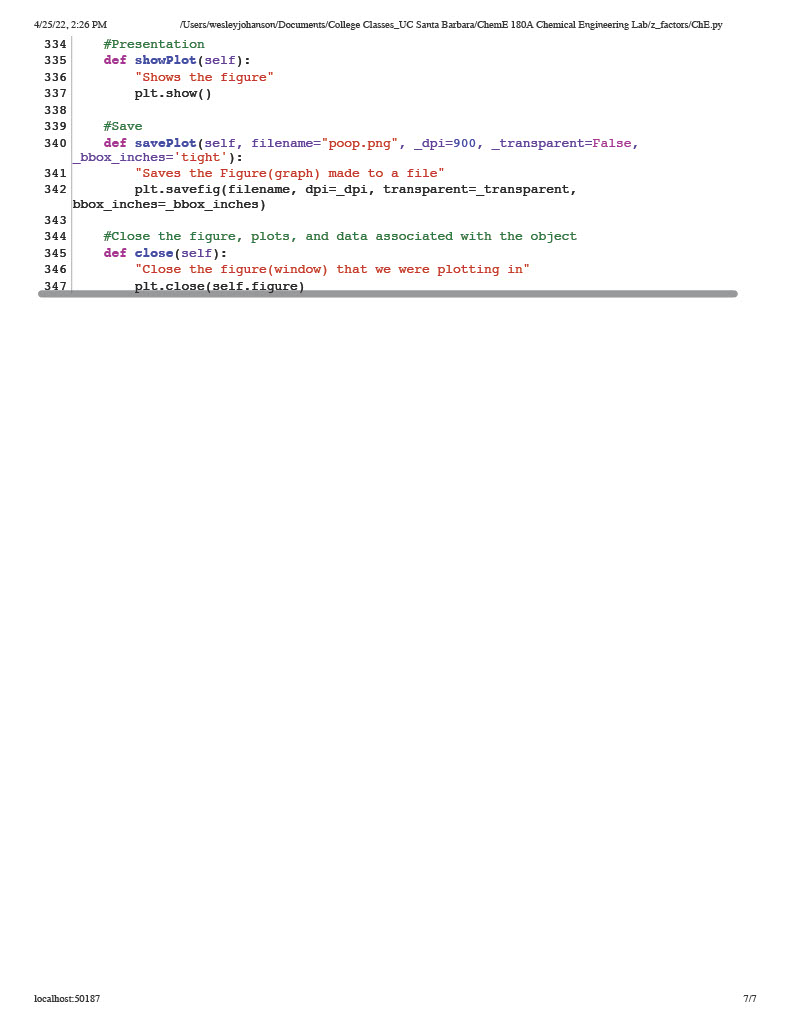
\includegraphics[width=0.8\textwidth]{code/che_py1024_7.jpg}
\caption{\label{fig1}Plotting Class python code}\end{figure}


%END  ______________________________________________________________
\end{document}

